% Choose one to switch between slides and handout
\documentclass[]{beamer}
%\documentclass[handout]{beamer}

% Video Meta Data
\title{Bitcoin, Blockchain and Cryptoassets}
\subtitle{Bitcoin Script Transaction Types}
\author{Prof. Dr. Fabian Schär}
\institute{University of Basel}

% Config File
% Packages
\usepackage[utf8]{inputenc}
\usepackage{hyperref}
\usepackage{gitinfo2}
\usepackage{tikz}
\usepackage{amsmath}
\usepackage{bibentry}
\usepackage{xcolor}
\usepackage{colortbl} % Add colour to LaTeX tables
\usepackage{caption}
\usepackage[export]{adjustbox}
\usepackage{pgfplots} \pgfplotsset{compat = 1.17}

% Color Options
\definecolor{highlight}{rgb}{0.65,0.84,0.82}
\definecolor{focus}{rgb}{0.72, 0, 0}

% Beamer Template Options
\beamertemplatenavigationsymbolsempty
\setbeamertemplate{footline}[frame number]
\setbeamercolor{structure}{fg=black}
\setbeamercolor{footline}{fg=black}
\setbeamercolor{title}{fg=black}
\setbeamercolor{frametitle}{fg=black}
\setbeamercolor{item}{fg=black}
\setbeamercolor{}{fg=black}
\setbeamercolor{bibliography item}{fg=black}
\setbeamercolor*{bibliography entry title}{fg=black}
\setbeamertemplate{items}[square]
\setbeamertemplate{enumerate items}[default]
\captionsetup[figure]{labelfont={color=black},font={color=black}}
\captionsetup[table]{labelfont={color=black},font={color=black}}

\setbeamertemplate{bibliography item}{\insertbiblabel}

% Link Icon Command
\newcommand{\link}{%
    \tikz[x=1.2ex, y=1.2ex, baseline=-0.05ex]{%
        \begin{scope}[x=1ex, y=1ex]
            \clip (-0.1,-0.1)
                --++ (-0, 1.2)
                --++ (0.6, 0)
                --++ (0, -0.6)
                --++ (0.6, 0)
                --++ (0, -1);
            \path[draw,
                line width = 0.5,
                rounded corners=0.5]
                (0,0) rectangle (1,1);
        \end{scope}
        \path[draw, line width = 0.5] (0.5, 0.5)
            -- (1, 1);
        \path[draw, line width = 0.5] (0.6, 1)
            -- (1, 1) -- (1, 0.6);
        }
    }

% Read Git Data from Github Actions Workflow
% Defaults to gitinfo2 for local builds
\IfFileExists{gitInfo.txt}
	{\input{gitInfo.txt}}
	{
		\newcommand{\gitRelease}{(Local Release)}
		\newcommand{\gitSHA}{\gitHash}
		\newcommand{\gitDate}{\gitAuthorIsoDate}
	}

% Custom Titlepage
\defbeamertemplate*{title page}{customized}[1][]
{
  \vspace{-0cm}\hfill
\includegraphics[width=2.5cm]{../config/logo_cif}
  
\includegraphics[width=1.9cm]{../config/seal_wwz}
  \\ \vspace{2em}
  \usebeamerfont{title}\textbf{\inserttitle}\par
  \usebeamerfont{title}\usebeamercolor[fg]{title}\insertsubtitle\par  \vspace{1.5em}
  \small\usebeamerfont{author}\insertauthor\par
  \usebeamerfont{author}\insertinstitute\par \vspace{2em}
  \usebeamercolor[fg]{titlegraphic}\inserttitlegraphic
    \tiny \noindent \texttt{Release Ver.: \gitRelease}\\ 
    \texttt{Version Hash: \gitSHA}\\
    \texttt{Version Date: \gitDate}\\ \vspace{1em}
  \link \href{https://github.com/cifunibas/Bitcoin-Blockchain-Cryptoassets/blob/main/slides/intro.pdf}
  {Get most recent version}\\
  \link \href{https://github.com/cifunibas/Bitcoin-Blockchain-Cryptoassets/blob/main/slides/intro.pdf}
  {Watch video lecture}\\ \vspace{1em}
  License: \texttt{Creative Commons Attribution-NonCommercial-ShareAlike 4.0 International}\\\vspace{2em}
  
\includegraphics[width = 1.2cm]{../config/license}
}

% tikzlibraries
\usetikzlibrary{decorations.pathreplacing}
\usetikzlibrary{decorations.markings}
\usetikzlibrary{positioning}

%caption font
\captionsetup{font=footnotesize}

\usepackage{fancybox}
\usepackage{ragged2e}

%%%%%%%%%%%%%%%%%%%%%%%%%%%%%%%%%%%%%%%%%%%%%%
%%%%%%%%%%%%%%%%%%%%%%%%%%%%%%%%%%%%%%%%%%%%%%
\begin{document}


%%%
\thispagestyle{empty}
\begin{frame}[noframenumbering]
	\titlepage
\end{frame}
%%%


%%%
\begin{frame}{Unlocking Condition and \texttt{Script}}
\begin{itemize}
	\item Unlocking conditions are written and verified in \texttt{Script}.\\
	 $\rightarrow$ Scripting-Language with predetermined list of commands, called $OP\ Codes$.
	 \item Is based on the stacking principle. (Last in First out)
	 \item Only if all commands run through without errors and the end result of the stack is a \texttt{1} (\texttt{TRUE}), the transaction is considered valid.
	 \item Does not contain any loops, as these enable potential attack vectors.
\end{itemize}
\end{frame}
%%%


%%%
\begin{frame}{\texttt{scriptPubKey} and \texttt{scriptSig} in Transactions}
\begin{figure}
	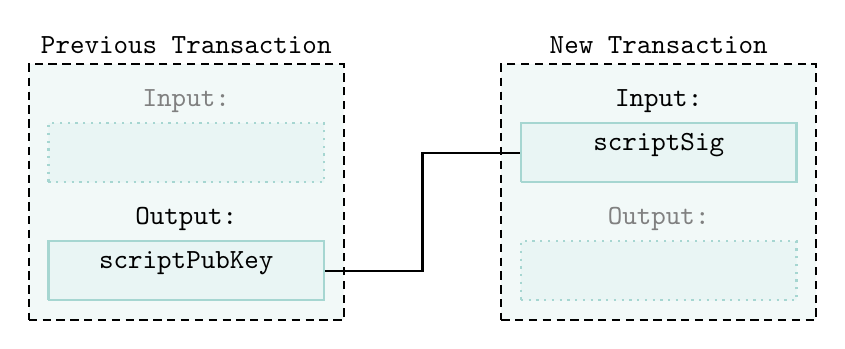
\begin{tikzpicture}[scale=1]
    \draw[densely dashed, thick, fill=highlight!15] (0,0) -- (4,0) -- (4,3.25) -- (0,3.25) node[midway,above]{{\texttt{Previous Transaction}}} -- (0,0);
    \draw[densely dashed, thick, fill=highlight!15] (6,0) -- (10,0) -- (10,3.25) -- (6,3.25) node[midway,above]{{\texttt{New Transaction}}} -- (6,0);
    
  \draw[thick,black] (3.75,0.625) -- (5,0.625) -- (5,2.125) -- (6.25, 2.125);
    
    \draw[color = highlight, fill = highlight!25, thick] (0.25,0.25) -- (3.75,0.25) -- (3.75,1) -- (0.25, 1) node[midway,above,color=black]{{\texttt{Output:}}}  node[below,midway,color=black]{\texttt{scriptPubKey}} -- (0.25,0.25);
      \draw[color = highlight, dotted, fill = highlight!25, thick] (0.25,1.75) -- (3.75,1.75) -- (3.75,2.5) -- (0.25, 2.5) node[midway,above,color=black!50]{{\texttt{Input:}}} -- (0.25,1.75);
      
    \draw[color = highlight, dotted, fill = highlight!25, thick] (6.25,0.25) -- (9.75,0.25) -- (9.75,1) -- (6.25, 1) node[midway,above,color=black!50]{{\texttt{Output:}}} -- (6.25,0.25);
      \draw[color = highlight, fill = highlight!25, thick] (6.25,1.75) -- (9.75,1.75) -- (9.75,2.5) -- (6.25, 2.5) node[midway,above,color=black]{{\texttt{Input:}}} node[below,midway,color=black]{\texttt{scriptSig}} -- (6.25,1.75);   
  \end{tikzpicture}
\end{figure}
\end{frame}
%%%


%%%
\begin{frame}{Pay-to-Public-Key}
\shadowbox{
\begin{minipage}[c]{4.1in}
\texttt{scriptSig: <sig>}\\
\texttt{scriptPubKey: <pubKey> OP\_CHECKSIG}
\end{minipage}
}
\vspace{1em}
\begin{itemize}
	\item{Pay-to-Public-Key links output directly to the public key.}
	\item{Solution (\texttt{scriptSig}) only includes corresponding signature (\texttt{<sig>}).}
	\item{Public key (\texttt{<pubKey>}) is deposited as part of the unlocking condition.}
\end{itemize}
\end{frame}
%%%


%%%
\begin{frame}{P2PK}
\begin{figure}
\centering
\begin{tikzpicture}[scale=1, every node/.style={scale=1.45}]  %,domain=0:8

%Stack
\draw[very thick] (-0.1,0) -- (4.1,0);
\draw[very thick] (-0.1,0) -- (-0.1,4);
\draw[very thick] (4.1,0) -- (4.1,4);
\draw (2,-0.5) node[below] {\texttt{Stack}};

%Boxes
\only<1-3>{
\draw[color=black] plot (2,1)   node[minimum width=2.7cm,fill=highlight!15, thick, draw=highlight,below, rotate = 0] {\texttt{<sig>}};
  }

\only<2,3>{
\draw[color=black] plot (2,2)   node[minimum width=2.7cm,fill=focus!15, thick,  draw=focus,below, rotate = 0] {\texttt{<pubKey>}};
}

\only<3,4>{
\draw[color=black] plot (6.1,5)   node[minimum width=2.7cm, minimum height= 0.55cm ,fill=black!15, thick,  draw=black,below, rotate = 0] {\texttt{OP\_CHECKSIG}};
}

\only<4|handout:0>{
\draw[color=black] plot (2,5)   node[minimum width=2.7cm,fill=focus!15, thick,  draw=focus,below, rotate = 0] {\texttt{<pubKey>}};
}

\only<4|handout:0>{
\draw[color=black] plot (2,4)   node[minimum width=2.7cm,fill=highlight!15, thick,  draw=highlight,below, rotate = 0] {\texttt{<sig>}};
}

\only<5|handout:0>{
\draw[color=black] plot (2,0.9)   node[minimum width=2.7cm,fill=highlight!15, thick,  draw=highlight,below, rotate = 0] {\texttt{1}};
}

%Dummy
\only<1,2,5|handout:0>{
\draw[color=white] plot (6.1,5)   node[minimum width=2.7cm,fill=white, thick,  draw=white,below, rotate = 0] {\texttt{Dummy}};
}

\end{tikzpicture}
\end{figure}
\end{frame}
%%%


%%%
\begin{frame}{Pay-to-Address / Pay-to-Public-Key-Hash}
\shadowbox{
\begin{minipage}[c]{4.1in}
\texttt{scriptSig: <sig> <pubKey>}\\
\texttt{scriptPubKey: OP\_DUP OP\_HASH160 <pubKeyHash> OP\_EQUALVERIFY OP\_CHECKSIG}
\end{minipage}
}
\vspace{1em}
\begin{itemize}
	\item<2-> Output is linked to Bitcoin address instead of public key.
	\item<3-> Reference of an output with this unlocking condition only valid if the \texttt{scriptSig} contains:
	
	\begin{enumerate}
	 \item<4-> The public key (\texttt{<pubKey>}) associated with the address.
	 \item<4-> A matching signature (\texttt{<sig>}), derived from the underlying private key.
	\end{enumerate}
\end{itemize}
\end{frame}
%%%


%%%
\begin{frame}{P2PKH}
	
\begin{figure}
\centering
\begin{tikzpicture}[scale=1, every node/.style={scale=1.4}]  %,domain=0:8

%Stack
\draw[very thick] (-0.1,0) -- (4.1,0);
\draw[very thick] (-0.1,0) -- (-0.1,4);
\draw[very thick] (4.1,0) -- (4.1,4);
\draw (2,-0.5) node[below] {\texttt{Stack}};

%Boxes
\only<1-14>{
\draw[color=black] plot (2,1)   node[minimum width=2.7cm,fill=highlight!15, thick, draw=highlight,below, rotate = 0] {\texttt{<sig>}};
  }
  
\only<1,2,5-14>{
\draw[color=black] plot (2,2)   node[minimum width=2.7cm,fill=highlight!15, thick,  draw=highlight,below, rotate = 0] {\texttt{<pubKey>}};
}

\only<5,6|handout:0>{
\draw[color=black] plot (2,3)   node[minimum width=2.7cm, fill=highlight!15, thick,  draw=highlight,below, rotate = 0] {\texttt{<pubKey>}};
}

%OP Codes
\only<2,3|handout:0>{
\draw[color=black] plot (6.3,5)   node[minimum width=3.1cm, minimum height= 0.55cm ,fill=black!15, thick,  draw=black,below, rotate = 0] {\texttt{OP\_DUP}};
}

\only<6,7|handout:0>{
\draw[color=black] plot (6.3,5)   node[minimum width=3.1cm, minimum height= 0.55cm ,fill=black!15, thick,  draw=black,below, rotate = 0] {\texttt{OP\_HASH160}};
}

\only<11,12>{
\draw[color=black] plot (6.3,5)   node[minimum width=3.1cm, minimum height= 0.55cm , fill=black!15, thick,  draw=black,below, rotate = 0] {\texttt{OP\_EQUALVERIFY}};
}

\only<14,15|handout:0>{
\draw[color=black] plot (6.3,5)   node[minimum width=3.1cm, minimum height= 0.55cm , fill=black!15, thick,  draw=black,below, rotate = 0] {\texttt{OP\_CHECKSIG   }};
}

%Boxes 2
\only<3,4,7|handout:0>{
\draw[color=black] plot (2,5)   node[minimum width=2.7cm,fill=highlight!15, thick,  draw=highlight,below, rotate = 0] {\texttt{<pubKey>}};
}

\only<4|handout:0>{
\draw[color=black] plot (2,4)   node[minimum width=2.7cm,fill=highlight!15, thick,  draw=highlight,below, rotate = 0] {\texttt{<pubKey>}};
}

\only<8,12>{
\draw[color=black] plot (2,5)   node[minimum width=2.7cm,fill=highlight!15, thick,  draw=highlight,below, rotate = 0] {\texttt{<pubKeyHash>}};
}

\only<9,10,11|handout:0>{
\draw[color=black] plot (2,3)   node[minimum width=2.7cm,fill=highlight!15, thick,  draw=highlight,below, rotate = 0] {\texttt{<pubKeyHash>}};
}

\only<10,11|handout:0>{
\draw[color=black] plot (2,4)   node[minimum width=2.7cm,fill=focus!15, thick,  draw=focus,below, rotate = 0] {\texttt{<pubKeyHash>}};
}

\only<12>{
\draw[color=black] plot (2,5)   node[minimum width=2.7cm,fill=focus!15, thick,  draw=focus,below, rotate = 0] {\texttt{<pubKeyHash>}};
}

\only<12>{
\draw[color=black] plot (2,4)   node[minimum width=2.7cm,fill=highlight!15, thick,  draw=highlight,below, rotate = 0] {\texttt{<pubKeyHash>}};
}

\only<15|handout:0>{
\draw[color=black] plot (2,5)   node[minimum width=2.7cm,fill=highlight!15, thick,  draw=highlight,below, rotate = 0] {\texttt{<pubKey>}};
}

\only<15|handout:0>{
\draw[color=black] plot (2,4)   node[minimum width=2.7cm,fill=highlight!15, thick,  draw=highlight,below, rotate = 0] {\texttt{<sig>}};
}

\only<16|handout:0>{
\draw[color=black] plot (2,0.9)   node[minimum width=2.7cm,fill=highlight!15, thick,  draw=highlight,below, rotate = 0] {\texttt{1}};
}

%Dummy
\only<1,4,5,8,9,10,13,16|handout:0>{
\draw[color=white] plot (6.3,5)   node[minimum width=3.1cm,fill=white, thick,  draw=white,below, rotate = 0] {\texttt{OP\_HASH160}};
}

\end{tikzpicture}

%%%%%%%%%%%%%%%% Stack %%%%%%%%%%%%%%%%%%%%%%%%%%%%%%%%
%\draw[very thick] (0,0) -- (4,0);
%\draw[very thick] (0,0) -- (0,4);
%\draw[very thick] (4,0) -- (4,4);
%\draw (2,-0.5) node[below] {\texttt{Stack}};

%%%%%%%%%%%%%%%% Nodes %%%%%%%%%%%%%%%%%%%%%%%%%%%%%%%

%  \draw[color=black] plot (0,-1)   node[minimum width=2.7cm,fill=highlight!15, thick, draw=highlight,below, rotate = 0] {\texttt{<sig>}};
  
%  \draw[color=black] plot (0,0)   node[minimum width=2.7cm,fill=highlight!15, thick,  draw=highlight,below, rotate = 0] {\texttt{<pubKey>}};

%	\draw[color=black] plot (2.1,2.55)   node[minimum width=2.7cm,fill=black!15, thick,  draw=black,right, rotate = 0] {\texttt{<OP\_DUB>}};  
   
%  \draw[color=black] plot (0,3)   node[minimum width=2.7cm,fill=highlight!15, thick,  draw=highlight,below, rotate = 0] {\texttt{<pubKey>}};
 
	
%  \draw[color=black] plot (0,2)   node[minimum width=2.7cm,fill=highlight!15, thick,  draw=highlight,below, rotate = 0] {\texttt{<pubKeyHash>}};

%  \draw[color=black] plot (0,3)   node[minimum width=2.7cm,fill=highlight!15, thick,  draw=highlight,below, rotate = 0] {\texttt{<pubKeyH>}};
  
%%%%%%%%%%%%%% OP_Code %%%%%%%%%%%%%%%%%%%%%%%%%%%%%%%%%%%
  
%  \draw[color=black] plot (2.1,2.55)   node[minimum width={width("Magnetometer")+2pt},fill=black!15, thick,  draw=black,right, rotate = 0] {\texttt{<OP\_EQUALVERIFY>}};

%  \draw[color=black] plot (2.1,2.55)   node[minimum width={width("Magnetometer")+2pt},fill=black!15, thick,  draw=black,right, rotate = 0] {\texttt{<OP\_HASH160>}};  

%  \draw[color=black] plot (2.1,2.55)   node[minimum width={width("Magnetometer")+2pt},fill=black!15, thick,  draw=black,right, rotate = 0] {\texttt{<OP\_DUP>}};    
\end{figure}

\end{frame}
%%% 

%%%
\begin{frame}{Multisig (M of N)}
\shadowbox{
\begin{minipage}[c]{4.1in}
\texttt{scriptSig: OP\_0 <sig1> <sig2>}\\
\texttt{scriptPubKey: M <pubKey1>\dots<pubKeyN> N {OP\_CHECKMULTISIG}}
\end{minipage}
}
\vspace{1em}
\begin{itemize}
  \item Enables payout conditions that require $M$ of $N$ signatures to reference the corresponding transaction output.
  \item<2-> Unlocking condition (\texttt{scriptPubKey}) includes $N$ public keys.
  \item<3-> At least $M$ of the corresponding private keys must provide a valid signature in \texttt{scriptSig}.
  \item<4-> Applications include increasing the security of funds and the possibility of imitating classic bank accounts (joint account, corporate account).
\end{itemize}
\end{frame}
%%%


%%%
\begin{frame}{Pay-to-Multisig (2 out of 3 Script)}
\centering
\begin{tikzpicture}[scale=1, every node/.style={scale=1}]  %,domain=0:8

%Stack
\draw[very thick] (0.5,0) -- (3.5,0);
\draw[very thick] (0.5,0) -- (0.5,5.5);
\draw[very thick] (3.5,0) -- (3.5,5.5);
\draw (2,-0.3) node[below] {\texttt{Stack}};

%Boxes
\only<1-5>{
\draw[color=black] plot (2,0.6)   node[minimum width=2.7cm,fill=highlight!15, thick, draw=highlight,below, rotate = 0] {\texttt{OP\_0}};
  }
  
\only<1-5>{
\draw[color=black] plot (2,1.3)   node[minimum width=2.7cm,fill=highlight!15, thick,  draw=highlight,below, rotate = 0] {\texttt{<sig 1>}};
}

\only<1-5>{
\draw[color=black] plot (2,2)   node[minimum width=2.7cm, fill=highlight!15, thick,  draw=highlight,below, rotate = 0] {\texttt{<sig 2>}};
}

\only<2-4>{
\draw[color=black] plot (2,2.7)   node[minimum width=2.7cm, minimum height= 0.55cm, fill=focus!15, thick,  draw=focus,below, rotate = 0] {\texttt{m <2>}};
}

\only<2,3>{
\draw[color=black] plot (2,3.4)   node[minimum width=2.7cm,fill=focus!15, thick,  draw=focus,below, rotate = 0] {\texttt{<pubKey 1>}};
}

\only<2,3>{
\draw[color=black] plot (2,4.1)   node[minimum width=2.7cm,fill=focus!15, thick,  draw=focus,below, rotate = 0] {\texttt{<pubKey 2>}};
}

\only<2,3>{
\draw[color=black] plot (2,4.8)   node[minimum width=2.7cm, fill=focus!15, thick,  draw=focus,below, rotate = 0] {\texttt{<pubKey 3>}};
}

\only<2>{
\draw[color=black] plot (2,5.5)   node[minimum width=2.7cm, minimum height= 0.55cm, fill=focus!15, thick,  draw=focus,below, rotate = 0] {\texttt{n <3>}};
}

\only<2-10>{
\draw[color=black] plot (5.3,6.2)   node[minimum width=2.7cm, minimum height= 0.55cm , fill=black!15, thick,  draw=black,below, rotate = 0] {\texttt{OP\_CHECKMULTISIG}};
}

\only<3-10>{
\draw[color=black] plot (2,6.2)   node[minimum width=2.7cm, minimum height= 0.55cm, fill=focus!15, thick,  draw=focus,below, rotate = 0] {\texttt{n <3>}};
}

\only<4-9>{
\draw[color=black] plot (2,4.1)   node[minimum width=2.7cm,fill=focus!15, thick,  draw=focus,below, rotate = 0] {\texttt{<pubKey 1>}};
}

\only<10>{
\draw[color=black] plot (2,4.1)   node[minimum width=2.7cm,fill=black!15, thick,  draw=black,below, rotate = 0] {\texttt{<pubKey 1>}};
}

\only<4-8>{
\draw[color=black] plot (2,4.8)   node[minimum width=2.7cm,fill=focus!15, thick,  draw=focus,below, rotate = 0] {\texttt{<pubKey 2>}};
}

\only<9,10>{
\draw[color=black] plot (2,4.8)   node[minimum width=2.7cm,fill=black!15, thick,  draw=black,below, rotate = 0] {\texttt{<pubKey 2>}};
}

\only<4-9>{
\draw[color=black] plot (2,5.5)   node[minimum width=2.7cm, fill=focus!15, thick,  draw=focus,below, rotate = 0] {\texttt{<pubKey 3>}};
}

\only<8-10>{
\draw[color=black] plot (2,5.5)   node[minimum width=2.7cm, fill=black!15, thick,  draw=black,below, rotate = 0] {\texttt{<pubKey 3>}};
}

\only<5-10>{
\draw[color=black] plot (2,3.4)   node[minimum width=2.7cm, minimum height= 0.55cm, fill=focus!15, thick,  draw=focus,below, rotate = 0] {\texttt{m <2>}};
}

\only<6-9>{
\draw[color=black] plot (2,2)   node[minimum width=2.7cm,fill=highlight!15, thick,  draw=highlight,below, rotate = 0] {\texttt{<sig 1>}};
}

\only<10>{
\draw[color=black] plot (2,2)   node[minimum width=2.7cm,fill=black!15, thick,  draw=black,below, rotate = 0] {\texttt{<sig 1>}};
}

\only<6-8>{
\draw[color=black] plot (2,2.7)   node[minimum width=2.7cm, fill=highlight!15, thick,  draw=highlight,below, rotate = 0] {\texttt{<sig 2>}};
}

\only<9-10>{
\draw[color=black] plot (2,2.7)   node[minimum width=2.7cm, fill=black!15, thick,  draw=black,below, rotate = 0] {\texttt{<sig 2>}};
}

\only<6-9>{
\draw[color=black] plot (2,1.3)   node[minimum width=2.7cm,fill=highlight!15, thick, draw=highlight,below, rotate = 0] {\texttt{OP\_0}};
  }
  
  
\only<10>{
\draw[color=black] plot (2,1.3)   node[minimum width=2.7cm,fill=black!15, thick, draw=black,below, rotate = 0] {\texttt{OP\_0}};
  }
  
%Lines, Checkmarks & Counters (Checkmultisig)  
\only<7>{
\draw[->, color=black, dashed] (0.3,2.4) -- (0.6,2.4);
\draw[color=black, dashed] (0.3,2.4) -- (0.3,5.2);
\draw[color=black, dashed] (0.3,5.2) -- (0.6,5.2);
\draw (0.3,3.8) node[left] {X};
\draw (3.7,3.1) node[right] {0/2};
}

\only<8>{
\draw[->, color=black, dashed] (0.3,2.4) -- (0.6,2.4);
\draw[color=black, dashed] (0.3,2.4) -- (0.3,4.5);
\draw[color=black, dashed] (0.3,4.5) -- (0.6,4.5);
\draw (0.4,3.45) node[left] {$\checkmark$};
\draw (3.7,3.1) node[right] {1/2};
}

\only<9>{
\draw[->, color=black, dashed] (0.3,1.7) -- (0.6,1.7);
\draw[color=black, dashed] (0.3,1.7) -- (0.3,3.8);
\draw[color=black, dashed] (0.3,3.8) -- (0.6,3.8);
\draw (0.4,2.75) node[left] {$\checkmark$};
\draw (3.7,3.1) node[right] {2/2};
}

\only<10>{
\draw (7,5.9) node[right] {$\checkmark$};
\draw (3.7,3.1) node[right] {2/2};
}

%True
\only<11>{
\draw[color=black] plot (2,0.6)   node[minimum width=2.7cm,fill=highlight!15, thick, draw=highlight,below, rotate = 0] {\texttt{1}};
}

%Dummy 1
\only<1-11>{
\draw[color=white] (0.3,0.7) -- (0.3,1.0);
\draw[color=white] (0.3,0.7) node[left] {X};
}

%Dummy 2
\only<1,11>{
\draw[color=white] plot (5.3,6.2)   node[minimum width=2.7cm, minimum height= 0.55cm , fill=white!15, thick,  draw=white,below, rotate = 0] {\texttt{OP\_CHECKMULTISIG}};
}

%Dummy 3
\only<1-9,11>{
\draw[color=white] (7,5.9) node[right] {$\checkmark$};
}


\end{tikzpicture}
\end{frame}
%%%


%%%
\begin{frame}{Pay-to-Script-Hash (Flexible Scripts)}
\shadowbox{
\begin{minipage}[c]{4.1in}
\texttt{scriptSig: }Any valid script\\
\texttt{scriptPubKey: {OP\_HASH160 <scriptHash> OP\_EQUALVERIFY}}
\end{minipage}
}
  \vspace{1em}
\begin{itemize}
  \item<1-> In the \texttt{scriptPubKey}, only the hash value of a script is recorded.
  \item<2-> To reference the transaction output, a person must provide a \texttt{scriptSig} whose hash value corresponds to the hash value set in the \texttt{scriptPubKey}.
  \item<3-> If this succeeds, the complete script of the \texttt{scriptSig} is run through in the second step.
\end{itemize}
\end{frame}
%%%


%%%
\begin{frame}{P2SH}
\centering
\begin{figure}
	\begin{tikzpicture}[scale=1, every node/.style={scale=1}]  %,domain=0:8

%Stack
\only<1-11>{
\draw[very thick] (5,0) -- (8,0);
\draw[very thick] (5,0) -- (5,5.5);
\draw[very thick] (8,0) -- (8,5.5);
\draw (6.5,-0.3) node[below] {\texttt{Stack}};
}

%Copy Stack
\only<3-11>{
\draw[color=black!20, very thick] (0.5,0) -- (3.5,0);
\draw[color=black!20, very thick] (0.5,0) -- (0.5,5.5);
\draw[color=black!20, very thick] (3.5,0) -- (3.5,5.5);
\draw[color=black!20] (2,-0.3) node[below] {\texttt{Copy}};
}

%Boxes
\only<1-11>{
\draw[color=black] plot (6.5,0.7)   node[minimum width=2.7cm,fill=highlight!15, thick,  draw=highlight,below, rotate = 0] {\texttt{<sig Y>}};

\draw[color=black] plot (6.5,1.4)   node[minimum width=2.7cm, fill=highlight!15, thick,  draw=highlight,below, rotate = 0] {\texttt{<sig X>}};
}

\only<2-5>{
\draw[color=black] plot (6.5,2.1)   node[minimum width=2.7cm, fill=highlight!15, thick,  draw=highlight,below, rotate = 0] {\texttt{<script>}};
}

\only<3-11>{
\draw[color=black!20] plot (2,0.7)   node[minimum width=2.7cm,fill=highlight!5, thick,  draw=highlight!50,below, rotate = 0] {\texttt{<sig Y>}};

\draw[color=black!20] plot (2,1.4)   node[minimum width=2.7cm, fill=highlight!5, thick,  draw=highlight!50,below, rotate = 0] {\texttt{<sig X>}};

\draw[color=black!20] plot (2,2.1)   node[minimum width=2.7cm, fill=highlight!5, thick,  draw=highlight!50,below, rotate = 0] {\texttt{<script>}};
}

\only<4,5>{
\draw[color=black] plot (9.5,6.2)   node[minimum width=2.7cm, minimum height= 0.55cm ,fill=black!15, thick,  draw=black,below, rotate = 0] {\texttt{OP\_HASH160}};
}

\only<5|handout:0>{
\draw[color=black] plot (6.5,6.2)   node[minimum width=2.7cm, fill=highlight!15, thick,  draw=highlight,below, rotate = 0] {\texttt{<script>}};
}

\only<6|handout:0>{
\draw[color=black] plot (6.5,6.2)   node[minimum width=2.7cm, fill=highlight!15, thick,  draw=highlight,below, rotate = 0] {\texttt{<scriptHash>}};
}

\only<7,8,9|handout:0>{
\draw[color=black] plot (6.5,2.1)   node[minimum width=2.7cm, fill=highlight!15, thick,  draw=highlight,below, rotate = 0] {\texttt{<scriptHash>}};
}

\only<8,9|handout:0>{
\draw[color=black] plot (6.5,2.8)   node[minimum width=2.7cm, fill=focus!15, thick,  draw=focus,below, rotate = 0] {\texttt{<scriptHash>}};
}

\only<9,10|handout:0>{
\draw[color=black] plot (9.5,6.2)   node[minimum width=2.7cm, minimum height= 0.55cm ,fill=black!15, thick,  draw=black,below, rotate = 0] {\texttt{OP\_EQUAL  }};
}

\only<10|handout:0>{
\draw[color=black] plot (6.5,6.2)   node[minimum width=2.7cm, fill=focus!15, thick,  draw=focus,below, rotate = 0] {\texttt{<scriptHash>}};
\draw[color=black] plot (6.5,5.5)   node[minimum width=2.7cm, fill=highlight!15, thick,  draw=highlight,below, rotate = 0] {\texttt{<scriptHash>}};
}

\only<11|handout:0>{
\draw[color=black] plot (6.5,2.1)   node[minimum width=2.7cm, minimum height= 0.55cm, fill=highlight!15, thick,  draw=highlight,below, rotate = 0] {\texttt{1}};
}

%Copy Stack 2
\only<12|handout:0>{
\draw[very thick] (0.5,0) -- (3.5,0);
\draw[very thick] (0.5,0) -- (0.5,5.5);
\draw[very thick] (3.5,0) -- (3.5,5.5);
\draw (2,-0.3) node[below] {\texttt{Copy}};

%Stack 2
\draw[color=black!20, very thick] (5,0) -- (8,0);
\draw[color=black!20, very thick] (5,0) -- (5,5.5);
\draw[color=black!20, very thick] (8,0) -- (8,5.5);
\draw[color=black!20] (6.5,-0.3) node[below] {\texttt{Stack}};

%more Boxes
\draw[color=black] plot (2,0.7)   node[minimum width=2.7cm,fill=highlight!15, thick,  draw=highlight,below, rotate = 0] {\texttt{<sig Y>}};

\draw[color=black] plot (2,1.4)   node[minimum width=2.7cm, fill=highlight!15, thick,  draw=highlight,below, rotate = 0] {\texttt{<sig X>}};

\draw[color=black!20] plot (6.5,0.7)   node[minimum width=2.7cm,fill=highlight!5, thick,  draw=highlight!50,below, rotate = 0] {\texttt{<sig Y>}};

\draw[color=black!20] plot (6.5,1.4)   node[minimum width=2.7cm, fill=highlight!5, thick,  draw=highlight!50,below, rotate = 0] {\texttt{<sig X>}};

\draw[color=black!20] plot (6.5,2.1)   node[minimum width=2.7cm, minimum height= 0.55cm, fill=highlight!5, thick,  draw=highlight!50,below, rotate = 0] {\texttt{1}};

\draw[color=black] plot (2,2.1)   node[minimum width=2.7cm, fill=highlight!15, thick,  draw=highlight,below, rotate = 0] {\texttt{<script>}};
}

%another Stack
\only<13|handout:0>{
\draw[color=black, very thick] (0.5,0) -- (3.5,0);
\draw[color=black, very thick] (0.5,0) -- (0.5,5.5);
\draw[color=black, very thick] (3.5,0) -- (3.5,5.5);
\draw[color=black] (2,-0.3) node[below] {\texttt{Stack}};
}

\only<13|handout:0>{
\draw[color=black] plot (2,0.7)   node[minimum width=2.7cm,fill=highlight!15, thick,  draw=highlight,below, rotate = 0] {\texttt{<sig 2>}};

\draw[color=black] plot (2,1.4)   node[minimum width=2.7cm, fill=highlight!15, thick,  draw=highlight,below, rotate = 0] {\texttt{<sig 3>}};

\draw[color=black] plot (2,2.1)   node[minimum width=2.7cm, fill=highlight!15, thick,  draw=highlight,below, rotate = 0] {\texttt{<script>}};
}

%% Dummy Stack
\only<13|handout:0>{
\draw[color=white, very thick] (5,0) -- (8,0);
\draw[color=white, very thick] (5,0) -- (5,5.5);
\draw[color=white, very thick] (8,0) -- (8,5.5);
\draw[color=white] (6.5,-0.3) node[below] {\texttt{Stack}};
}

%% Dummy OPCODE
\only<1-3,6-8,11-13|handout:0>{
\draw[color=white] plot (9.5,6.2)   node[minimum width=2.7cm, minimum height=0.55cm ,fill=white, thick,  draw=white, below, rotate = 0] {\texttt{OP\_HASH160}};
}

\end{tikzpicture}
\end{figure}
\end{frame}
%%%


%%%
\begin{frame}{Characteristics and Risks of Pay-to-Script-Hash}
\begin{itemize}
	\item<1-> By using the cryptographically secure hash value, it can be ensured that the unlocking condition can only be solved using the previously specified script.
	\item<2-> High degree of flexibility, as Bitcoin units can be collateralised by a wide variety of scripts.
	\item<3-> Scripts only need to be submitted at the time of a transaction. %(reduce amount of data and prevent complex and long scripts from becoming part of a non-used transaction output).
	\item<4-> Can be represented as a kind of Bitcoin address with prefix 3. %Enables uncomplicated payment orders analogous to classic Bitcoin addresses.
	\vspace{1em}
	\item<5-> Possible problems: 
	\begin{itemize}
  \item<5-> P2SH addresses based on invalid scripts.
  \item<5-> Loss of payout script.
\end{itemize}\vspace{0.5em}
$\Rightarrow$ Both result in loss of Bitcoin units.
\end{itemize}
\end{frame}
%%%


%%%
\begin{frame}{Null Data (\texttt{OP\_RETURN)}}
\shadowbox{
\begin{minipage}[c]{4.1in}
\texttt{scriptSig: }Non-existent.\\
\texttt{scriptPubKey: {OP\_RETURN <0 to 40 Bytes of Data>}}
\end{minipage}
}
\begin{itemize}
  \item<1-> Null Data unlocking conditions are not really transactions.
  \item<2-> Used to immortalise arbitrary data up to 40 bytes (320 bits) in the blockchain.
  \item<3-> Possible applications: 
    \begin{itemize}
      \item<3-> \textit{Proof-of-Existence}: Proof that a certain file existed at a certain point in time. For this purpose, the hash value of a file is stored in the blockchain using a zero data transaction.
      \item<3-> Many \textit{Colored Coin} implementations also use the additional data to identify the linked promises to pay.
    \end{itemize}
\end{itemize}
\end{frame}
%%%




\end{document}
